\documentclass[handout]{beamer}
\setbeamertemplate{footline}[frame number]

%\AtBeginDocument{%
%  \pdfpageheight = \paperheight
%  \pdfpagewidth = \paperwidth
%}

\usepackage{txfonts}
\usepackage{tree-dvips}
\usepackage{color}
\usepackage{latexsym}
\usepackage{graphicx}
\ifx\pdfoutput\undefined
  \usepackage{graphicx}
\else
  %\usepackage[pdftex]{graphicx}
  \DeclareGraphicsRule{*}{mps}{*}{}
\fi
%\usepackage{cgloss4e,gb4e}

\raggedright

\definecolor{bgblue}{rgb}{0.04,0.39,0.53}

\newcommand{\argmax}[1]{\begin{array}{c}\mbox{arg max}\\#1\end{array}}

\begin{document}


\title{\color{blue}Natural Language Processing}

\author{Anoop Sarkar \\ {\tt http://anoopsarkar.github.io/nlp-class}}
\institute{}
%\date{}
     
{
\setbeamertemplate{navigation symbols}{}
\addtocounter{framenumber}{-1}
\begin{frame}
\begin{center}
\vspace{1cm}

\includegraphics[scale=0.4]{figures/natlang-cky-logo.eps}
\end{center}
\titlepage
\end{frame}
}



\begin{frame}[fragile]
\frametitle{Probabilistic CFG (PCFG)}
\[
\begin{array}{cccc}
 S & \rightarrow & NP~VP  & 1 \\
 VP & \rightarrow & V~NP  & 0.9 \\
 VP & \rightarrow & VP~PP & 0.1 \\
 PP & \rightarrow & P~NP  & 1 \\
 NP & \rightarrow & NP~PP & 0.25 \\
 NP & \rightarrow & Calvin  & 0.25 \\
 NP & \rightarrow & monsters & 0.25 \\
 NP & \rightarrow & school & 0.25 \\
 V & \rightarrow & imagined  &  1 \\
 P & \rightarrow & in     & 1
\end{array}
\]
\begin{eqnarray}
&P(\textit{input}) = \sum_{\textit{tree}} P(\textit{tree} \mid \textit{input}) \nonumber\\
&P(\textit{Calvin imagined monsters in school}) = ? \nonumber\\
&\textrm{Notice that } P(VP \rightarrow V~NP) + P(VP \rightarrow VP~PP) = 1.0 \nonumber
\end{eqnarray}
\end{frame}

\begin{frame}[fragile]
\frametitle{Probabilistic CFG (PCFG)}
\[ P(\textit{Calvin imagined monsters in school}) = ? \]
\begin{verbatim}
(S (NP Calvin)
   (VP (V imagined)
       (NP (NP monsters)
           (PP (P in)
               (NP school)))))

(S (NP Calvin)
   (VP (VP (V imagined)
           (NP monsters))
       (PP (P in)
           (NP school))))
\end{verbatim}

\end{frame}

\begin{frame}[fragile]
\frametitle{Probabilistic CFG (PCFG)}
\begin{verbatim}
(S (NP Calvin)
   (VP (V imagined)
       (NP (NP monsters)
           (PP (P in)
               (NP school)))))
\end{verbatim}
{\small
\begin{eqnarray*}
P(\textit{tree$_1$})& = & P(S \rightarrow NP\ VP) \times
      P(NP \rightarrow Calvin) \times
      {\color{red} P(VP \rightarrow V\ NP)} \times \nonumber \\
&& P(V \rightarrow imagined) \times 
   {\color{blue} P(NP \rightarrow NP\ PP)} \times
   P(NP \rightarrow monsters) \times \nonumber \\
&& P(PP \rightarrow P\ NP) \times  
   P(P \rightarrow in) \times  
   P(NP \rightarrow school) \nonumber \\
& = & 1 \times 0.25 \times {\color{red} 0.9} \times 1 \times {\color{blue} 0.25} \times 0.25 \times 1 \times 1 \times 0.25 = .003515625 \nonumber 
\end{eqnarray*}
}
\end{frame}

\begin{frame}[fragile]
\frametitle{Probabilistic CFG (PCFG)}
\begin{verbatim}
(S (NP Calvin)
   (VP (VP (V imagined)
           (NP monsters))
       (PP (P in)
           (NP school))))
\end{verbatim}
{\small
\begin{eqnarray*}
P(\textit{tree$_2$})& = & P(S \rightarrow NP\ VP) \times
      P(NP \rightarrow Calvin) \times
      {\color{blue} P(VP \rightarrow VP\ PP)} \times \nonumber \\
&& {\color{red} P(VP \rightarrow V\ NP)} \times
   P(V \rightarrow imagined) \times 
   P(NP \rightarrow monsters) \times \nonumber \\
&& P(PP \rightarrow P\ NP) \times  
   P(P \rightarrow in) \times  
   P(NP \rightarrow school) \nonumber \\
& = & 1 \times 0.25 \times {\color{blue} 0.1} \times {\color{red} 0.9} \times 1 \times 0.25 \times 1 \times 1 \times 0.25 = .00140625 \nonumber 
\end{eqnarray*}
}
\end{frame}

\begin{frame}[fragile]
\frametitle{Probabilistic CFG (PCFG)}
\begin{eqnarray}
P(\textit{Calvin imagined monsters in school}) & = &
P(\textit{tree$_1$}) + P(\textit{tree$_2$}) \nonumber\\ 
& = & .003515625 + .00140625 \nonumber \\
& = & .004921875 \nonumber\\
\textrm{Most likely tree is \textit{tree$_1$}} & = & \argmax{\textit{tree}} P(\textit{tree} \mid \textit{input}) \nonumber
\end{eqnarray}
\bigskip
\begin{minipage}{4in}
\begin{verbatim}
(S (NP Calvin)
   (VP (V imagined)
       (NP (NP monsters)
           (PP (P in)
               (NP school)))))
\end{verbatim}
\end{minipage}
\begin{minipage}{4in}
\begin{verbatim}
(S (NP Calvin)
   (VP (VP (V imagined)
           (NP monsters))
       (PP (P in)
           (NP school))))
\end{verbatim}
\end{minipage}

\end{frame}

\begin{frame}
\frametitle{PCFG}
\begin{itemize}
\item Central condition: \( \sum_\alpha P( A \rightarrow \alpha) = 1 \)
\item Called a {\em proper} PCFG if this condition holds
\item Note that this means $P( A \rightarrow \alpha) = P( \alpha \mid A) = \frac{f(A, \alpha)}{f(A)}$
\item \( P(T \mid S) = \frac{P(T,S)}{P(S)} = P(T,S) = \prod_i P(RHS_i \mid LHS_i) \)
\end{itemize}

\end{frame}

\begin{frame}
\frametitle{PCFG}
\begin{itemize}
\item What is the PCFG that can be extracted from this single tree: 
\begin{tabbing}
0123\=4567\=8901\=2345\=6789\=0123\=4567 \kill
(S \>(NP (Det the) (NP man)) \\
\> (VP \> (VP \> (V played) \\
\> \> \> (NP (Det a) (NP game))) \\
\> \> (PP \>(P with) \\
\> \> \> (NP (Det the) (NP dog)))))
\end{tabbing}
\item How many different rhs $\alpha$ exist for $A \rightarrow \alpha$ where $A$ can be {\it S, NP, VP, PP, Det, N, V, P}
\end{itemize}

\end{frame}

\begin{frame}
\frametitle{PCFG}
{\small
\[
\begin{array}{ccccll}
 S & \rightarrow & NP~VP  & c=1 & p = 1/1 & = 1.0 \\
 NP & \rightarrow & Det~NP & c=3 & p = 3/6 & = 0.5 \\
 NP & \rightarrow & man  & c=1 & p = 1/6 & = 0.1667 \\
 NP & \rightarrow & game  & c=1 & p = 1/6 & = 0.1667 \\
 NP & \rightarrow & dog  & c=1 & p = 1/6 & = 0.1667 \\
 VP & \rightarrow & VP~PP  & c=1 & p = 1/2 & = 0.5 \\
 VP & \rightarrow & V~NP  & c=1 & p = 1/2 & = 0.5 \\
 PP & \rightarrow & P~NP  & c=1 & p = 1/1 & = 1.0 \\
 Det & \rightarrow & the  & c=2 & p = 2/3 & = 0.67 \\
 Det & \rightarrow & a  & c=1 & p = 1/3 & = 0.33 \\
 V & \rightarrow & played & c=1 & p = 1/1 & = 1.0 \\
 P & \rightarrow & with & c=1 & p = 1/1 & = 1.0 \\
\end{array}
\] 
}
\begin{itemize}
\item We can do this with multiple trees. Simply count occurrences of CFG rules over all the trees. 
\item A repository of such trees labelled by a human is called a TreeBank.
\end{itemize}
\end{frame}


%\begin{frame}
%\frametitle{Parsing PCFGs: CKY algorithm $+$ Viterbi}
%{\small\begin{frame}
%$p: S \rightarrow S\ S\ ,\ 1-p: S \rightarrow a$
%\end{frame}}
%\begin{frame}
%\begin{tabular}{|c|c|c|c|}
%\hline
% a & a & a & a \\
%\hline
%$1-p$: S$_{0,1}$ $\rightarrow$ a & $1-p$: S$_{1,2}$ $\rightarrow$ a & $1-p$: S$_{2,3}$ $\rightarrow$ a & $1-p$: S$_{3,4}$ $\rightarrow$ a \\
%\hline
% S$_{0,1}$ $+$  S$_{1,2}$ & S$_{1,2}$ $+$  S$_{2,3}$ & S$_{2,3}$ $+$  S$_{3,4}$ & \\
% $=$ S$_{0,2}$ $\rightarrow$ S\ S & $=$ S$_{1,3}$ $\rightarrow$ S\ S & $=$ S$_{2,4}$ $\rightarrow$ S\ S & \\
% $p(1-p)^2$ & $p(1-p)^2$  & $p(1-p)^2$  & \\
%\hline
% S$_{0,1}$ $+$  S$_{1,3}$ & S$_{1,2}$ $+$  S$_{2,4}$ & & \\
% OR & OR & & \\
% S$_{0,2}$ $+$  S$_{2,3}$ &   S$_{1,3}$ $+$  S$_{3,4}$ & & \\
% $=$ S$_{0,3}$ $\rightarrow$ S\ S &  $=$ S$_{1,4}$ $\rightarrow$ S\ S & &\\
%$\textrm{max}(p^2(1-p)^3,$ & $\textrm{max}(p^2(1-p)^3,$ & & \\
%$p^2(1-p)^3)$ & $p^2(1-p)^3)$ & & \\
%\hline
% {\em What goes in this cell?} & & & \\
% ?? $=$ S$_{0,4}$ &&& \\
%\hline
%\end{tabular}
%\end{frame}
%
%\end{frame}

%\begin{frame}
%\frametitle{Example PCFG}
%\[
%\begin{array}{cccc}
% S & \rightarrow & NP~VP  & 1 \\
% VP & \rightarrow & V~NP  & 0.9 \\
% VP & \rightarrow & VP~PP & 0.1 \\
% PP & \rightarrow & P~NP  & 1 \\
% NP & \rightarrow & NP~PP & 0.25 \\
% NP & \rightarrow & Calvin  & 0.25 \\
% NP & \rightarrow & monsters & 0.25 \\
% NP & \rightarrow & school & 0.25 \\
% V & \rightarrow & imagined  &  1 \\
% P & \rightarrow & in     & 1
%\end{array}
%\] 
%
%\end{frame}

%\begin{frame}
%\frametitle{CKY Viterbi}
%\begin{frame}
%\begin{tabular}{|c|c|c|c|c|}
%\hline
% Calvin & imagined & monsters & in & school \\
%\hline
% NP$_{0,1}$ & V$_{1,2}$  &NP$_{2,3}$ &  P$_{3,4}$ &  NP$_{4,5}$ \\
%$0.25$ & $1$ & $0.25$ & $1$ & $0.25$ \\
%\hline
% & V$_{1,2}$ $+$  NP$_{2,3}$ & & P$_{3,4}$ $+$ NP$_{4,5}$ &\\
% & $=$ VP$_{1,3}$ $\rightarrow$ V\ NP & & $=$ PP$_{3,5}$ $\rightarrow$ P NP & \\
% & $1 \times 0.25 \times 0.9$  &  & $1^2 \times 0.25$ & \\
%\hline
%  &  VP$_{1,3}$ $+$ PP$_{3,5}$ & NP$_{2,3}$ $+$ PP$_{3,5}$ & & \\
% &   OR & $=$ NP$_{2,5}$ $\rightarrow$ NP PP  & &\\
% &   V$_{1,2}$ $+$ NP$_{2,5}$ & $0.25^3$  & &\\
%  &  $=$ VP$_{1,5}$   & & & \\
% & $x$ & &&\\
%\hline
% & && & \\
% $=$ S$_{0,4}$ &&& &\\
% $x \times 0.25$ &&& &\\
%\hline
%\end{tabular}
%\end{frame}
%
%\end{frame}

\begin{frame}
\frametitle{Ambiguity}
\begin{itemize}
  \item Part of Speech ambiguity\\
        {\tt saw} $\rightarrow$ {\color{red}noun}\\
        {\tt saw} $\rightarrow$ {\color{red}verb}
  \item Structural ambiguity: Prepositional Phrases\\
        {\tt I saw (the man) with the telescope}\\
        {\tt I saw (the man with the telescope)}
  \item Structural ambiguity: Coordination\\
        {\tt a program to promote safety in ((trucks) and (minivans))}\\
        {\tt a program to promote ((safety in trucks) and (minivans))}\\
        {\tt ((a program to promote safety in trucks) and (minivans))}
\end{itemize}

\end{frame}

\begin{frame}[fragile]
\frametitle{Ambiguity $\leftarrow$ attachment choice in alternative parses}
\includegraphics[scale=.6]{figures/figures.18}
\end{frame}

\begin{frame}
\frametitle{Parsing as a machine learning problem}
\begin{itemize}
\item<1-> $S = $ a sentence \\
      $T = $ a parse tree \\
A statistical parsing model defines $P(T \mid S)$
\item<2-> Find best parse: $\textrm{arg max}\atop{T}$ $P(T \mid S)$
\item<3-> $P(T \mid S) = \frac{P(T, S)}{P(S)} = P(T,S)$
\item<4-> Best parse: $\textrm{arg max}\atop{T}$ $P(T, S)$
\item<5-> e.g. for PCFGs: $P(T, S) = \prod_{i=1 \ldots n} P(\textrm{RHS}_i \mid \textrm{LHS}_i)$
\end{itemize}

\end{frame}

\newcommand{\code}[1]{\mbox{\tt #1}}

\begin{frame}
\frametitle{Adding Lexical Information to PCFG}
\centering
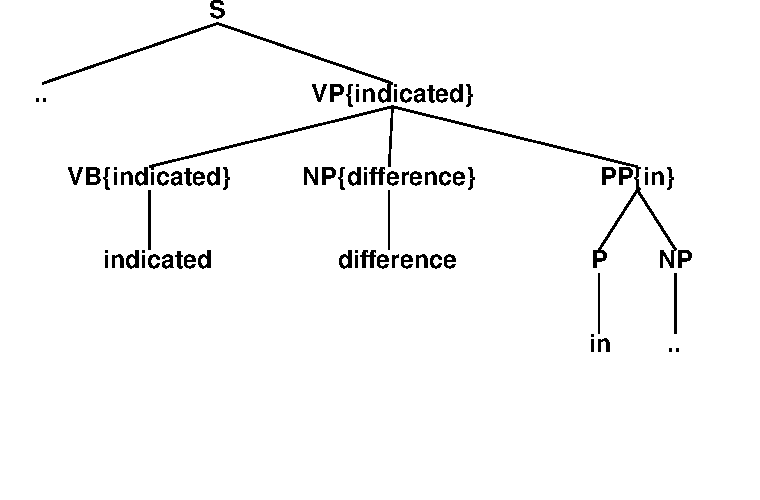
\includegraphics[scale=.7]{figures/bilexicalcfg0}
\end{frame}

\begin{frame}
\frametitle{Adding Lexical Information to PCFG {\footnotesize (Collins 99, Charniak 00)}}
\begin{center}
  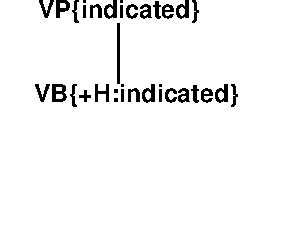
\includegraphics[scale=.5]{figures/bilexicalcfg1} \ 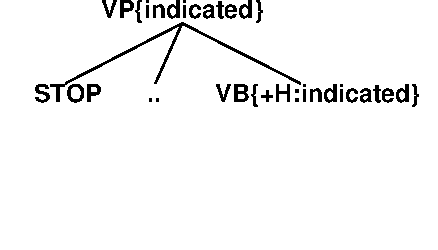
\includegraphics[scale=.5]{figures/bilexicalcfg2} \ 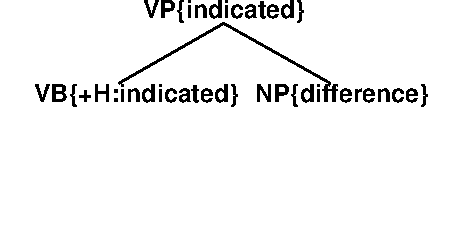
\includegraphics[scale=.5]{figures/bilexicalcfg3} 
\\ 
 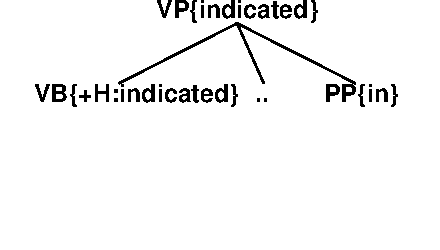
\includegraphics[scale=.5]{figures/bilexicalcfg4} \
 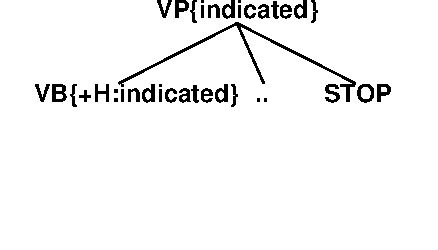
\includegraphics[scale=.5]{figures/bilexicalcfg5} 
\[ \begin{array}{l}
 P_h(\code{VB} \mid \code{VP}, \code{indicated}) \times 
 P_l(\code{STOP} \mid \code{VP}, \code{VB}, \code{indicated}) \times
 \\ 
 P_r(\code{NP(difference)} \mid \code{VP}, \code{VB},
 \code{indicated}) \times \\
 P_r(\code{PP(in)} \mid \code{VP}, \code{VB}, \code{indicated}) \times
 \\ 
 P_r(\code{STOP} \mid \code{VP}, \code{VB}, \code{indicated})
 \end{array} \]
\end{center}
\end{frame}

%\begin{frame}
%\frametitle{Adding Additional Features to PCFGs {\footnotesize (Collins 99)}}
%  \begin{center}
%  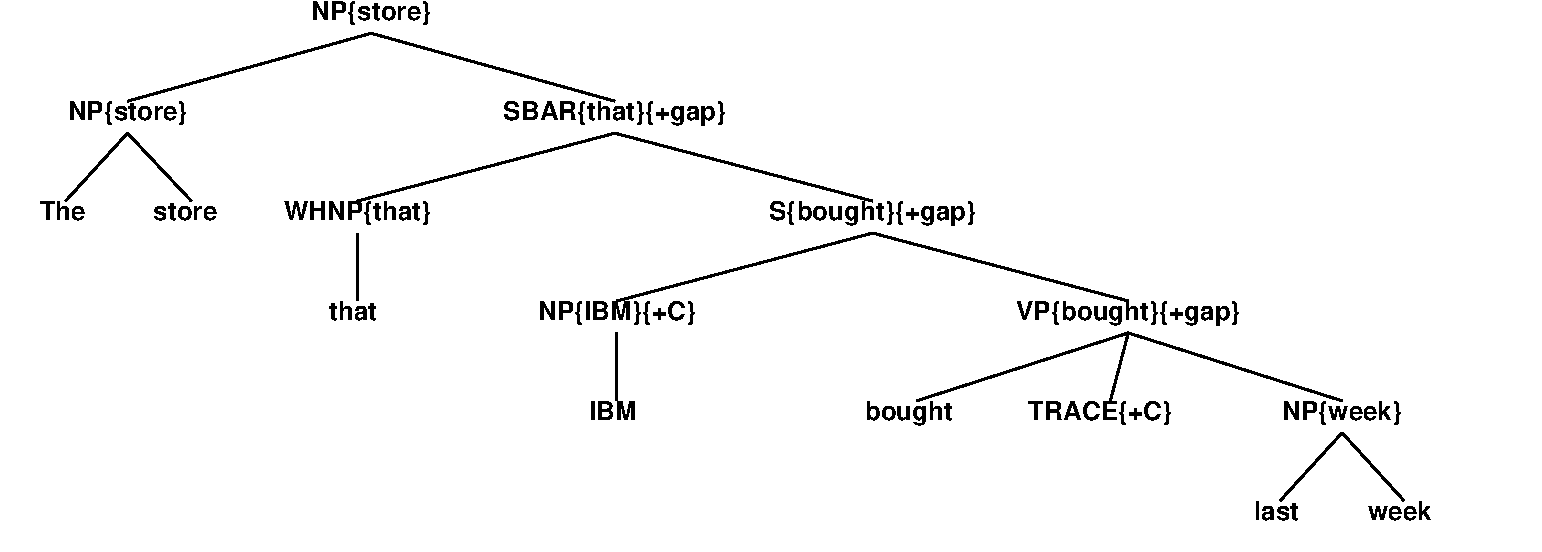
\includegraphics[scale=.4]{figures/cfgfeat}
%  \end{center}
%  {\footnotesize\tt
%  \begin{tabular}{lllllll}
%  NP           & $\rightarrow$ & [ & NP\{+H\}  & SBAR\{+gap\}          &    & ] \\
%  SBAR\{+gap\} & $\rightarrow$ & [ & WHNP      & S\{+H\}\{+C\}\{+gap\} &    & ] \\
%  S\{+gap\}    & $\rightarrow$ & [ & NP\{+C\}  & SBAR\{+H\}\{+gap\}    &    & ] \\
%  VP\{+gap\}   & $\rightarrow$ & [ & VB\{+H\}  & TRACE\{+C\}           & NP & ]
%  \end{tabular}}
%\end{frame}

\begin{frame}[fragile]
\frametitle{Evaluation of Parsing}
\begin{itemize}
\item Consider a candidate parse to be evaluated against the truth (or gold-standard parse):
{\footnotesize
\begin{verbatim}
candidate: (S (A (P this) (Q is)) (A (R a) (T test)))
gold:      (S (A (P this)) (B (Q is) (A (R a) (T test))))
\end{verbatim}
}
\item In order to evaluate this, we list all the constituents
{\small\begin{center}
\begin{tabular}{|l|l|}
\hline
Candidate & Gold \\
\hline
(0,4,S) & (0,4,S) \\
(0,2,A) & (0,1,A) \\
(2,4,A) & (1,4,B) \\
        & (2,4,A) \\
\hline
\end{tabular}
\end{center}
}
\item Skip spans of length 1 which would be equivalent to part of speech
tagging accuracy.
\item Precision is defined as $\frac{\#correct}{\#proposed} = \frac{2}{3}$
and recall as $\frac{\#correct}{\#in\ gold} = \frac{2}{4}$. 
\item Another measure: crossing brackets,
{\small\begin{verbatim}
candidate: [ an [incredibly expensive] coat ] (1 CB)
gold:      [ an [incredibly [expensive coat]]
\end{verbatim}
}
\end{itemize}
\end{frame}

\begin{frame}[fragile]
\frametitle{Evaluation of Parsing}
{\footnotesize
\[
\begin{array}{lcl}
\mbox{Bracketing recall}\ R & = & \frac{\mbox{num of correct constituents}}{\mbox{num of constituents in the goldfile}} \\
\\
\mbox{Bracketing precision}\ P & = & \frac{\mbox{num of correct constituents}}{\mbox{num of constituents in the parsed file}} \\
\\
\mbox{Complete match} & = & \mbox{\% of sents where recall \& precision are both 100\%} \\
\\
\mbox{Average crossing} & = & \frac{\mbox{num of constituents crossing a goldfile constituent}}{\mbox{num of sents}} \\
\\
\mbox{No crossing} & = & \mbox{\% of sents which have $0$ crossing brackets} \\
\\
\mbox{$2$ or less crossing} & = & \mbox{\% of sents which have $\leq 2$ crossing brackets}
\end{array}
\]
}
\end{frame}

\begin{frame}
\frametitle{Statistical Parsing Results}
\begin{center}
\footnotesize
\[ \textrm{F1-score} = 2 \frac{\textit{precision} \cdot \textit{recall}}{\textit{precision} + \textit{recall}} \]
\begin{tabular}{|p{7cm}|l|}
\hline
  & $\leq 100 wds$  \\
System & F1-score \\
\hline
Shift-Reduce (Magerman, 1995)   & 84.14 \\
PCFG with Lexical Features (Collins, 1999)    & 88.19 \\
PCFG with Lexical Features (Charniak, 1999)   & 89.54 \\
$n$-best Re-ranking (Collins, 2000)    & 89.74 \\
Unlexicalized Berkeley parser (Petrov et al, 2007) & 90.10 \\
$n$-best Re-ranking (Charniak and Johnson, 2005) & 91.02 \\
Tree-insertion grammars (Carreras, Collins, Koo, 2008) & 91.10 \\
Ensemble $n$-best Re-ranking (Johnson and Ural, 2010) & 91.49 \\
Forest Re-ranking (Huang, 2010) & 91.70 \\
\hline
Unlabeled Data with Self-Training (McCloskey et al, 2006) & 92.10 \\
\hline
\end{tabular}
\end{center}
\end{frame}

\begin{frame}
\frametitle{Practical Issues: Beam Thresholding and Priors}
\begin{itemize}
\item Probability of nonterminal $X$ spanning $j \ldots k$:
$N[X,j,k]$
\item Beam Thresholding compares $N[X,j,k]$ with every other $Y$
where $N[Y,j,k]$
\item But what should be compared?
\item Just the {\em inside probability}: $P(X \stackrel{*}{\Rightarrow} t_j
\ldots t_k)$?\\
written as $\beta(X, j, k)$
\item Perhaps $\beta(\mbox{\tt FRAG}, 0, 3) > \beta(\mbox{\tt NP}, 0,
3)$, but {\tt NP}s are much more likely than {\tt FRAG}s in general
\end{itemize}
\end{frame}

\begin{frame}
\frametitle{Practical Issues: Beam Thresholding and Priors}
\begin{itemize}
\item The correct estimate is the {\em outside probability}: 
\[ P(S \stackrel{*}{\Rightarrow} t_1 \ldots t_{j-1}\ X\ t_{k+1} \ldots
t_n) \]\\
written as $\alpha(X, j, k)$ 
\item Unfortunately, you can only compute $\alpha(X, j, k)$
efficiently after you finish parsing and reach $(S, 0, n)$
\end{itemize}
\end{frame}

\begin{frame}
\frametitle{Practical Issues: Beam Thresholding and Priors}
\begin{itemize}
\item To make things easier we multiply the prior probability $P(X)$
with the inside probability
\item In beam Thresholding we compare every new insertion of $X$ for
span $j, k$ as follows:\\
Compare $P(X) \cdot \beta(X,j,k)$ with the most probable $Y$ $P(Y) \cdot
\beta(Y,j,k)$
\item Assume $Y$ is the most probable entry in $j,k$, then we compare
\begin{eqnarray}
\textsf{beam} \cdot P(Y) \cdot \beta(Y,j,k) \label{eq:1} \\
P(X) \cdot \beta(X,j,k) \label{eq:2}
\end{eqnarray}
\item If $(\ref{eq:2}) < (\ref{eq:1})$ then we prune $X$ for this span $j,k$ 
\item \textsf{beam} is set to a small value, say 0.001 or even 0.01. 
\item As the beam value increases, the parser speed increases (since more entries are pruned).
\item A simpler (but not as effective) alternative to using the beam is to keep only the top $K$ entries for each span $j,k$
%\item Other more sophisticated methods are given in (Goodman 1997)
\end{itemize}
\end{frame}

\begin{frame}
\frametitle{Experiments with Beam Thresholding}
%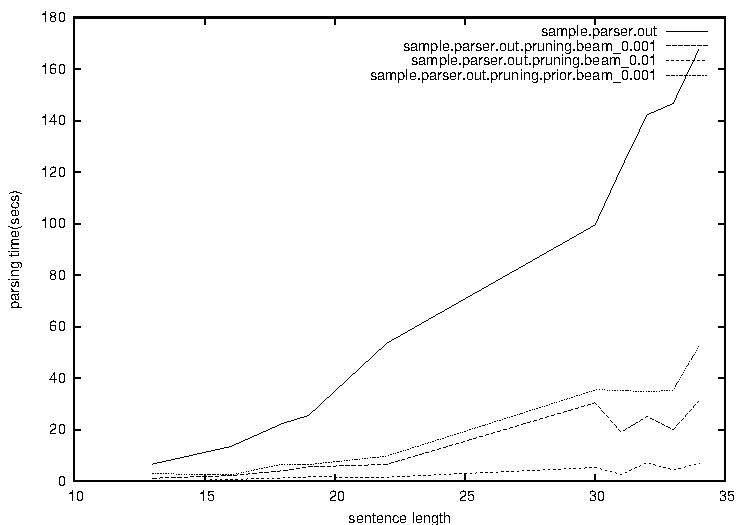
\includegraphics[scale=.85]{figures/parsetimes}
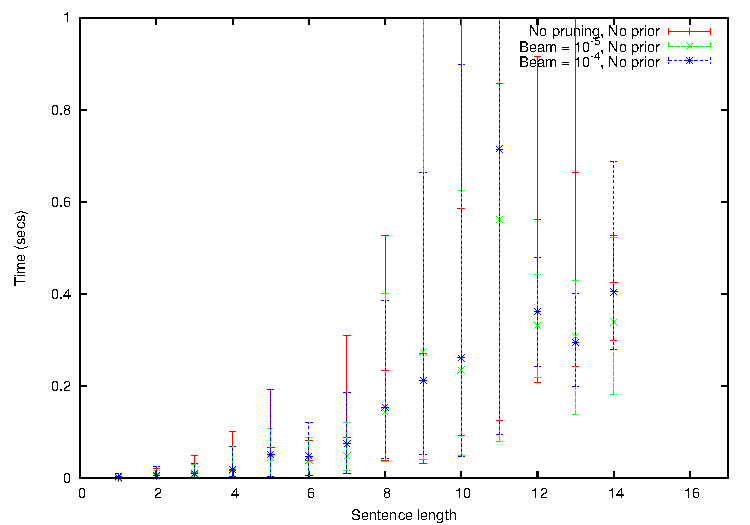
\includegraphics[scale=.85]{figures/timing-without-prior.pdf}
\end{frame}

\begin{frame}
\frametitle{Experiments with Beam Thresholding}
%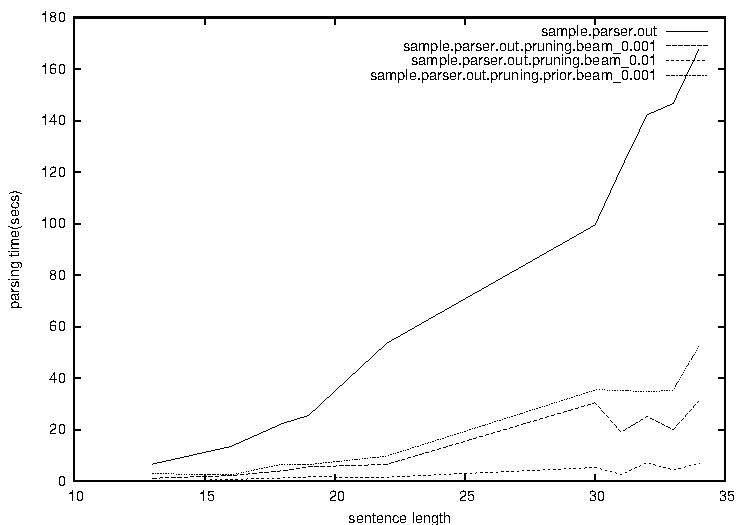
\includegraphics[scale=.85]{figures/parsetimes}
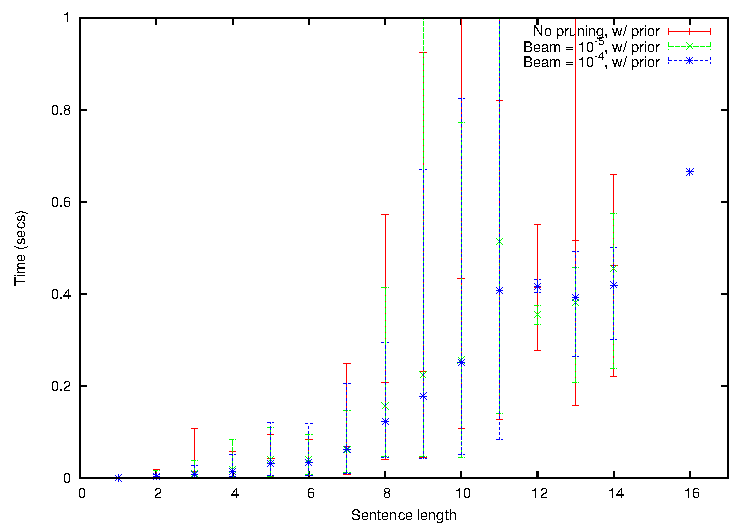
\includegraphics[scale=.85]{figures/timing-with-prior.pdf}
\end{frame}

\end{document}
